% Requires packages: booktabs, tikz
% Auto-generated polarization index report: run\_Phase2\_r1\_2026-05-25\_09-56-19
\begin{table}[ht]
\centering
\small
\begin{tabular}{llrrrr}
\toprule
Agent A & Agent B & WR(A,B) (\%) & |WR-50| & DeckStd & Polarization \\
\midrule
bazowy 21 & 21 glebokosciowy & 38.31 & 11.69 & 10.09 & 21.78\\
28 znormalizowany & 21 glebokosciowy & 38.88 & 11.12 & 10.54 & 21.66\\
63 parametry & 21 glebokosciowy & 37.93 & 12.07 & 8.80 & 20.86\\
63 plynny & 21 glebokosciowy & 38.92 & 11.08 & 9.41 & 20.49\\
28 parametrow & 21 glebokosciowy & 40.83 & 9.17 & 10.31 & 19.49\\
bazowy 21 & 28 parametrow & 46.52 & 3.48 & 9.28 & 12.77\\
28 parametrow & 28 znormalizowany & 52.60 & 2.60 & 10.13 & 12.73\\
63 plynny & 28 parametrow & 47.71 & 2.29 & 9.55 & 11.85\\
63 parametry & 28 parametrow & 46.46 & 3.54 & 8.01 & 11.55\\
bazowy 21 & 63 plynny & 48.64 & 1.36 & 8.71 & 10.06\\
bazowy 21 & 28 znormalizowany & 49.03 & 0.97 & 9.08 & 10.04\\
63 parametry & 28 znormalizowany & 49.06 & 0.94 & 8.59 & 9.53\\
63 plynny & 28 znormalizowany & 49.56 & 0.44 & 8.78 & 9.22\\
bazowy 21 & 63 parametry & 50.15 & 0.15 & 9.05 & 9.20\\
63 parametry & 63 plynny & 48.45 & 1.55 & 6.85 & 8.40\\
\bottomrule
\end{tabular}
\caption{Polarization index for run\_Phase2\_r1\_2026-05-25\_09-56-19: $\mathrm{PI}(A,B)=|WR(A,B)-50|+\sigma_{deck}(A,B)$. Higher = stronger and/or more deck-dependent matchup.}
\end{table}

\begin{figure}[ht]
\centering
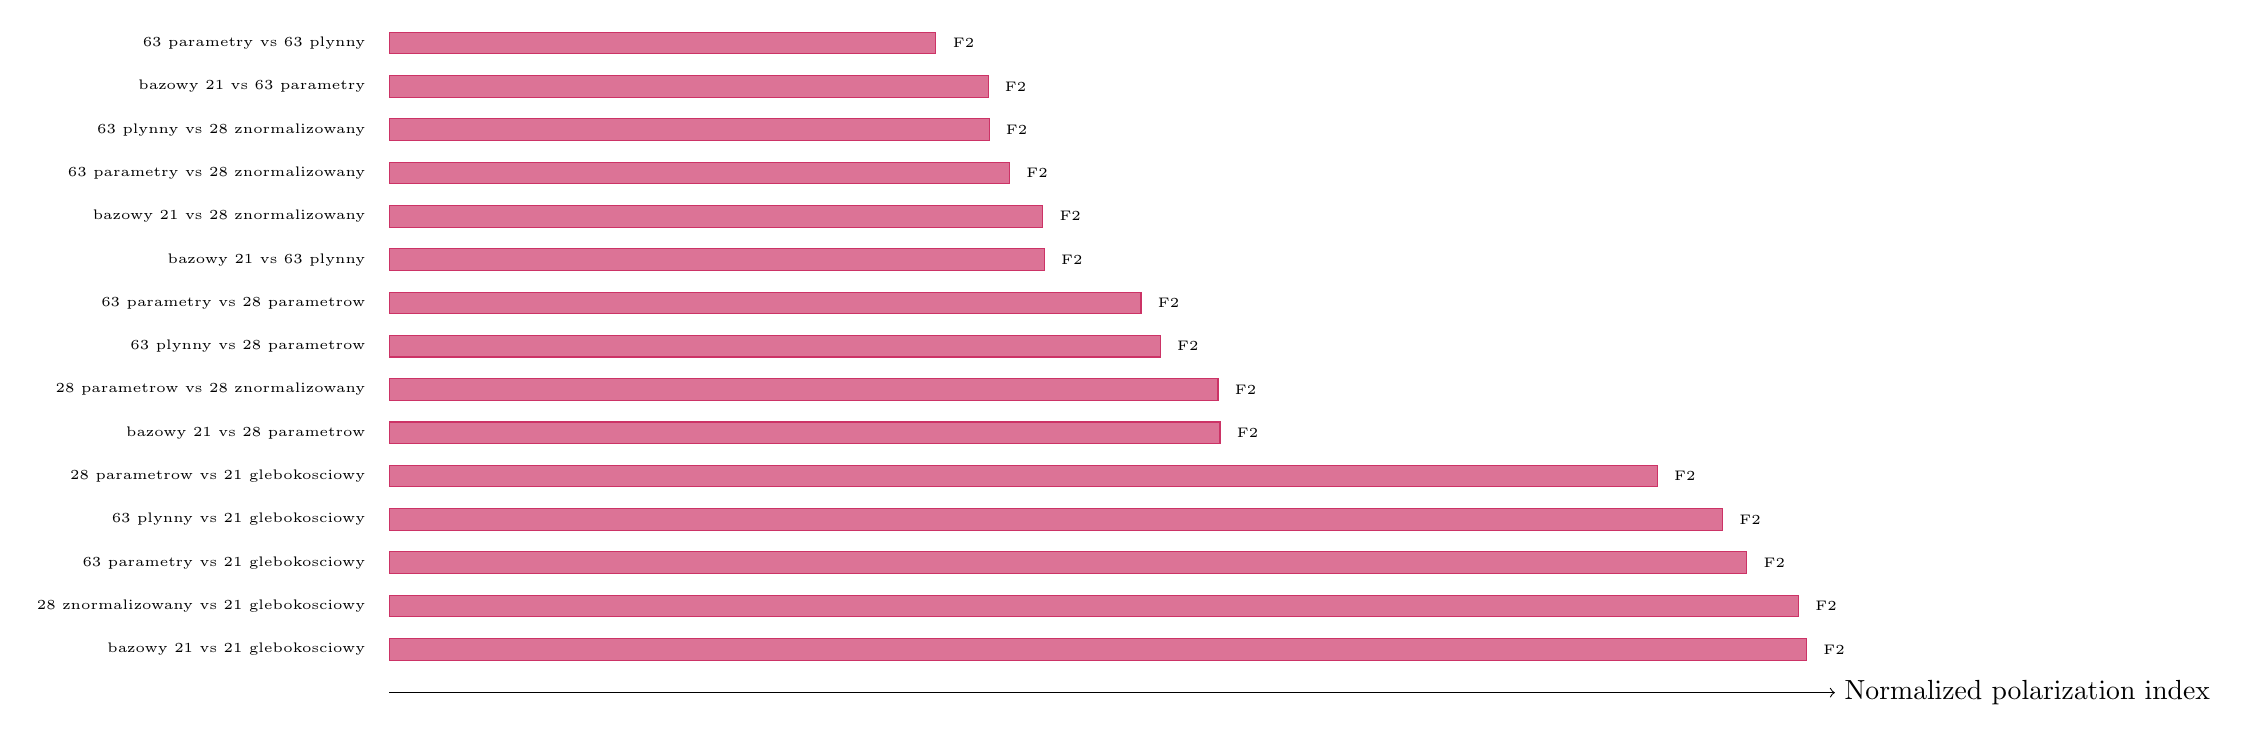
\begin{tikzpicture}[x=0.18cm,y=0.55cm]
\draw[->] (0,0) -- (102,0) node[right] {Normalized polarization index};
\filldraw[fill=purple!55, draw=purple!80] (0,1-0.25) rectangle (100.00,1+0.25);
\node[anchor=east, font=\tiny] at (-1,1) {bazowy 21 vs 21 glebokosciowy};
\node[anchor=west, font=\tiny] at (100.00+0.5,1) {F2};
\filldraw[fill=purple!55, draw=purple!80] (0,2-0.25) rectangle (99.43,2+0.25);
\node[anchor=east, font=\tiny] at (-1,2) {28 znormalizowany vs 21 glebokosciowy};
\node[anchor=west, font=\tiny] at (99.43+0.5,2) {F2};
\filldraw[fill=purple!55, draw=purple!80] (0,3-0.25) rectangle (95.79,3+0.25);
\node[anchor=east, font=\tiny] at (-1,3) {63 parametry vs 21 glebokosciowy};
\node[anchor=west, font=\tiny] at (95.79+0.5,3) {F2};
\filldraw[fill=purple!55, draw=purple!80] (0,4-0.25) rectangle (94.07,4+0.25);
\node[anchor=east, font=\tiny] at (-1,4) {63 plynny vs 21 glebokosciowy};
\node[anchor=west, font=\tiny] at (94.07+0.5,4) {F2};
\filldraw[fill=purple!55, draw=purple!80] (0,5-0.25) rectangle (89.46,5+0.25);
\node[anchor=east, font=\tiny] at (-1,5) {28 parametrow vs 21 glebokosciowy};
\node[anchor=west, font=\tiny] at (89.46+0.5,5) {F2};
\filldraw[fill=purple!55, draw=purple!80] (0,6-0.25) rectangle (58.61,6+0.25);
\node[anchor=east, font=\tiny] at (-1,6) {bazowy 21 vs 28 parametrow};
\node[anchor=west, font=\tiny] at (58.61+0.5,6) {F2};
\filldraw[fill=purple!55, draw=purple!80] (0,7-0.25) rectangle (58.47,7+0.25);
\node[anchor=east, font=\tiny] at (-1,7) {28 parametrow vs 28 znormalizowany};
\node[anchor=west, font=\tiny] at (58.47+0.5,7) {F2};
\filldraw[fill=purple!55, draw=purple!80] (0,8-0.25) rectangle (54.40,8+0.25);
\node[anchor=east, font=\tiny] at (-1,8) {63 plynny vs 28 parametrow};
\node[anchor=west, font=\tiny] at (54.40+0.5,8) {F2};
\filldraw[fill=purple!55, draw=purple!80] (0,9-0.25) rectangle (53.04,9+0.25);
\node[anchor=east, font=\tiny] at (-1,9) {63 parametry vs 28 parametrow};
\node[anchor=west, font=\tiny] at (53.04+0.5,9) {F2};
\filldraw[fill=purple!55, draw=purple!80] (0,10-0.25) rectangle (46.21,10+0.25);
\node[anchor=east, font=\tiny] at (-1,10) {bazowy 21 vs 63 plynny};
\node[anchor=west, font=\tiny] at (46.21+0.5,10) {F2};
\filldraw[fill=purple!55, draw=purple!80] (0,11-0.25) rectangle (46.10,11+0.25);
\node[anchor=east, font=\tiny] at (-1,11) {bazowy 21 vs 28 znormalizowany};
\node[anchor=west, font=\tiny] at (46.10+0.5,11) {F2};
\filldraw[fill=purple!55, draw=purple!80] (0,12-0.25) rectangle (43.76,12+0.25);
\node[anchor=east, font=\tiny] at (-1,12) {63 parametry vs 28 znormalizowany};
\node[anchor=west, font=\tiny] at (43.76+0.5,12) {F2};
\filldraw[fill=purple!55, draw=purple!80] (0,13-0.25) rectangle (42.32,13+0.25);
\node[anchor=east, font=\tiny] at (-1,13) {63 plynny vs 28 znormalizowany};
\node[anchor=west, font=\tiny] at (42.32+0.5,13) {F2};
\filldraw[fill=purple!55, draw=purple!80] (0,14-0.25) rectangle (42.25,14+0.25);
\node[anchor=east, font=\tiny] at (-1,14) {bazowy 21 vs 63 parametry};
\node[anchor=west, font=\tiny] at (42.25+0.5,14) {F2};
\filldraw[fill=purple!55, draw=purple!80] (0,15-0.25) rectangle (38.57,15+0.25);
\node[anchor=east, font=\tiny] at (-1,15) {63 parametry vs 63 plynny};
\node[anchor=west, font=\tiny] at (38.57+0.5,15) {F2};
\end{tikzpicture}
\caption{Polarization ranking for run\_Phase2\_r1\_2026-05-25\_09-56-19 (bars normalized to the maximum PI in this run).}
\end{figure}
